\documentclass{vldb}

%\usepackage{geometry} % see geometry.pdf on how to lay out the page. There's lots.
\usepackage{graphicx}
\usepackage{graphics}
\usepackage{lscape}
\usepackage{array}
\usepackage{enumerate}
\usepackage{url}
\usepackage{eufrak}
\usepackage{float}
\usepackage[colorlinks=true
,urlcolor=black
,anchorcolor=black
,citecolor=black
,filecolor=black
,linkcolor=black
,menucolor=black
,pagecolor=black]{hyperref}
\usepackage{algorithm}
\usepackage{algorithmic}
\usepackage{fancybox}
\usepackage{amsfonts}
\usepackage{amssymb}
\usepackage{amsmath}
\usepackage{verbatim}
\usepackage[table]{xcolor}
\usepackage{rotating}
\usepackage{subfig}
%\usepackage{program}
%\usepackage{amsthm}
\newcommand{\eat}[1]{}
% allows the coloring of the background of cells and rows in tables.  
% Use: \rowcolor[gray]{.80} or \cellcolor{grayL}
% also you can have colorfull text. For instance: 
% \textcolor{color}{words to be in color} 
\usepackage{color}
\usepackage{colortbl}
\definecolor{Brown}{cmyk}{0, 0.8, 1, 0.6}
%
\renewcommand{\algorithmicfor}{\textbf{foreach}}
\newcommand{\blackBox}{$\blacksquare$}
\newcommand{\qset}[1]{{\mathfrak{Constrs}}(#1)}
\newcommand{\ts}[2]{{\mathbb{TS}}_{#1}(#2)}
%\newcommand{\qset}[1]{{\mathfrak{Conds}}$$($$#1$$)$}
 



\DeclareCaptionType{copyrightbox}
\newdef{theorem}{Theorem}
\newdef{problem}{Problem definition}
\newtheorem{lemma}{Lemma}
\newtheorem{definition}{Definition}
\newtheorem{example}{Example}

\renewcommand{\algorithmicrequire}{\textbf{Input:}}
\renewcommand{\algorithmicensure}{\textbf{Output:}}


\begin{document}
\title{Spleetter: a PACT-based Twitter Statistical Analyzer}


\numberofauthors{2} 
\author{
\alignauthor
Matteo Lissandrini\\
       \affaddr{University of Trento}\\
%       \affaddr{UNITN}\\
       \email{{\small ml@disi.unitn.eu}}
\alignauthor
Davide Mottin\\
      \affaddr{University of Trento}\\
%       \affaddr{UNITN}\\
       \email{{\small mottin@disi.unitn.eu}}
}


\maketitle

\pagestyle{plain}
\pagenumbering{arabic}
\maketitle
%Abstract
\begin{abstract}
Twitter is the biggest micro-blogging system and users therein produce every day a 175 million of short messages\footnote{\url{http://www.mediabistro.com/alltwitter/twitter-stats_b32050}}, namely tweets.
The ability to perform analyses fast on the tweets is not only useful, but also vital to retrieve news and real-time statistics. 
However, since the number of different statistics to compute on the same data is big (e.g., the hashtag trend over the time, the number of tweets per user), there is the need of performing several operations at the same time. 
On one hand we can consider a Map-Reduce system in order to split the operations into different machines running several map and reduce steps.
On the other hand, a map and reduce paradigm may not suffice. 
We propose to solve this problem with a PACT flow, that is a semantically reacher map-reduce like-system.
Our solution is both simple and highly modular, being composed by simple operations that can be easily parallelised. 
We show how to compute a set of interesting statistics out of 22 million tweets downloaded in a period of two weeks, showing the polarity of each tweet and filtering the data to produce interesting analyses. 


\end{abstract}

% A category with the (minimum) three required fields
%\category{H.4}{Information Systems Applications}{Miscellaneous}
%%A category including the fourth, optional field follows...
%\category{D.2.8}{Software Engineering}{Metrics}[complexity measures, performance measures]
%
%\terms{Todo}
%
\keywords{Twitter, Stratosphere, Data Analysis, Sentiment Analysis}


%What you solved and how you solve it conceptually
%The data you used
%Screenshots and measurement results
%description of your  solution works (this should differ from the conceptual description)
%Criticism/problems you ran into

\section{Introduction}
\label{sec:introduction}
The ability to perform various statistical analyses with Twitter has attracted much interest and research in the last few years~\cite{Hong:2012qy,Lehmann:2012kx} and used to influence politics~\cite{Tumasjan:2010vn} and advertising~\cite{Bakshy:2011ys}. 
With 140 millions of users, Twitter is the leading social network for the real time sharing and re-sharing of information, having become the most used communication media in the spreading of socio-cultural events across the world
%~\footnote{\url{http://www.umpf.co.uk/blog/?p=6830}}
~\cite{DBLP:journals:corr:abs-1003-2664}. 
Moreover, Twitter has an enormous advantage over other social networks like Facebook in one key area: while people on Facebook tend to be friend their friends, users on Twitter subscribe to other users if they match their own interests\footnote{http://dcurt.is/twitters-graph}.
In~\cite{DBLP:journals:corr:abs-1003-2664,Mathioudakis:2010:EOI:1718487.1718525,DBLP:conf:chi:MarcusBBKMM11} authors introduce different techniques to identify peak of activities around particular keywords, \emph{hashtags} or users.
They describe topic discovery techniques to mine informative summarization of events, and to visualize user-friendly  streams of postings.
All these previous approaches aim to do real time identification of data peaks, smart labeling or even post-mortem analysis of events.

We would like to mine a real time stream of posts and to identify trends and patterns that allow us to forecast which topics, keywords or events will became popular in the near future.
For this reason, we need to gather social media timelines and to collect relevant statistics and insights on how events propagates in a social network.
However, the huge amount of information per day cannot be processed by a single machine.

To this end, we propose a schema based on the PACT paradigm implemented in Stratosphere, that is an enhanced map-reduce system able to mix second order functions. 
Our goal is to conduct an analysis of a big dataset, automatically downloaded using the Twitter streaming APIs.
We propose a PACT flow or program\footnote{here flow or program are used interchangeably} that takes in input a set of tuples, having tweets and user ids, a set of users and a vocabulary and produces several statistics used by data analysts in order to perform in-depth data analysis and event discovery. 
We now describe the basic structure of the Twitter system and a highlight of the proposed solution discussed in Section~\ref{sec:solution}. 

\subsection{Twitter structure}
Twitter is a micro-blogging system designed to allow users to send short messages having a maximum of 140 characters, called \textit{tweets}. 
In the text, users are allowed to specify \textit{hashtags} that are sequence of characters usually describing an argument and marked by the character '\#'. 
Users can also reference other users with '@user' notation. 
A particular kind of reference is a \textit{retweet} which is a tweet preceded by the tag ``RT'' and the user name that first posted the message. 
A user is \emph{retweeting} the tweet from another user when she thinks that it is an interesting piece of text to be shared her followers.
The last information in the tweets are the urls, that are usually shortened using available online services. 

\begin{table*}[!Ht]
\begin{tabular}{|l|l|l|}
\hline
tweet id & user id & tweet\\
\hline
292375792485298176&858488612& \#KidCudi - \#EraseMe - The Whizz Bells : http://t.co/Lp1zABOV via @youtube\\
292375792481099777&486970282& RT @Kirra\_\_: Today is a day where I need to crawl into my bed and sleep the day away.\\
292375792481099776&336390437& There are poor people, money is the only thing they got.\\
292375792476909568&74570186& I can't do anything without listening to music while I do it.\\
\hline
\end{tabular}
\caption{A sample of the tweet dataset}
\label{tbl:tweets}
\end{table*}


\subsection{Proposed solution}

We aim to find information regarding topic trends, analyzing user post trends, polarity of the tweets with respect to the creation time, and with respect also to hashtags contained in them. 
The set of operations we propose is the following:  
\begin{itemize}
\item \textbf{Tweet Cleansing}: we take in input the tuples containing the tweets and a dictionary of english words and we filter out hashtags, user mentions and tweets having a number of english words less than a threshold. The cleaned data are then used throughout the rest of the flow. 
\item \textbf{Polarity extraction}: we use a well-known library for sentiment analysis to extract the general polarity of each tweet. The polarity is defined as value in the range $[-5,5]$, where a positive number means that the user is talking about something in a favorable manner. Conversely, if a text has a negative polarity the text is written in a dissenting manner. 
We adopt the SentiStrength classifier (as in \cite{Thelwall:2010:SSS:1890706.1890713}) that was originally built to perform sentiment detection in short informal texts.
It combines a lexicon-based approach with more sophisticated linguistic rules.

%\item \textbf{User Analysis}: we analyse a bunch of statistics, such as the number of tweets per user, the number of 
% tweet per user/hashtag per user
\item \textbf{Hashtag analysis}: we produce a various statistics about hashtags. 
that take into account the time in which the hashtag appeared and disappeared (i.e. is not used anymore), the maximum and minimum number of mentions per hashtag with the timestamp of the peaks,  
\item \textbf{Topic Analysis}:  we perform an analysis of positive and negative per-topic trends, aggregating for each hashtag, for each point in time, the average polarity expressed in tweets containing it. 
We compute also the average Emotional Divergence\cite{DBLP:conf:icwsm:PfitznerGS12}  for each tag.
\end{itemize}

The document is structured as follows. Section~\ref{sec:data} describes the dataset we downloaded and used in our experiments. We propose a solution and describe the PACT program in detail in Section~\ref{sec:solution}. We also show the results of the analysis, with increasing size of the dataset in Section~\ref{sec:results}. Concluding, in Section~\ref{sec:issues} we describe the problems and the issues we encountered during the development of the solution and we remark our findings.

\section{Solution}
\label{sec:solution}

A PACT flow is 



\subsection{Data cleaning}

\begin{figure*}[t]
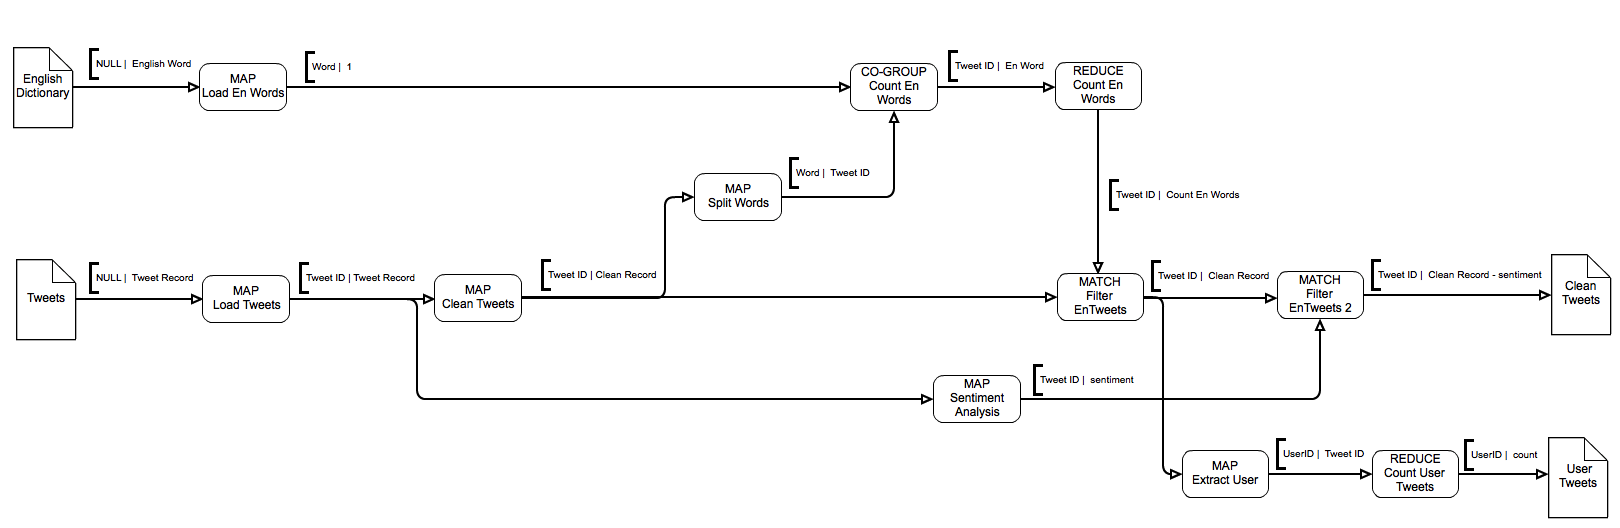
\includegraphics[width=\textwidth]{images/strato_pact_pt1.png} 
\caption{Data cleaning PACT}
\label{fig:cleaning}
\end{figure*}



\subsection{Compute statistics}

\begin{figure*}[t]
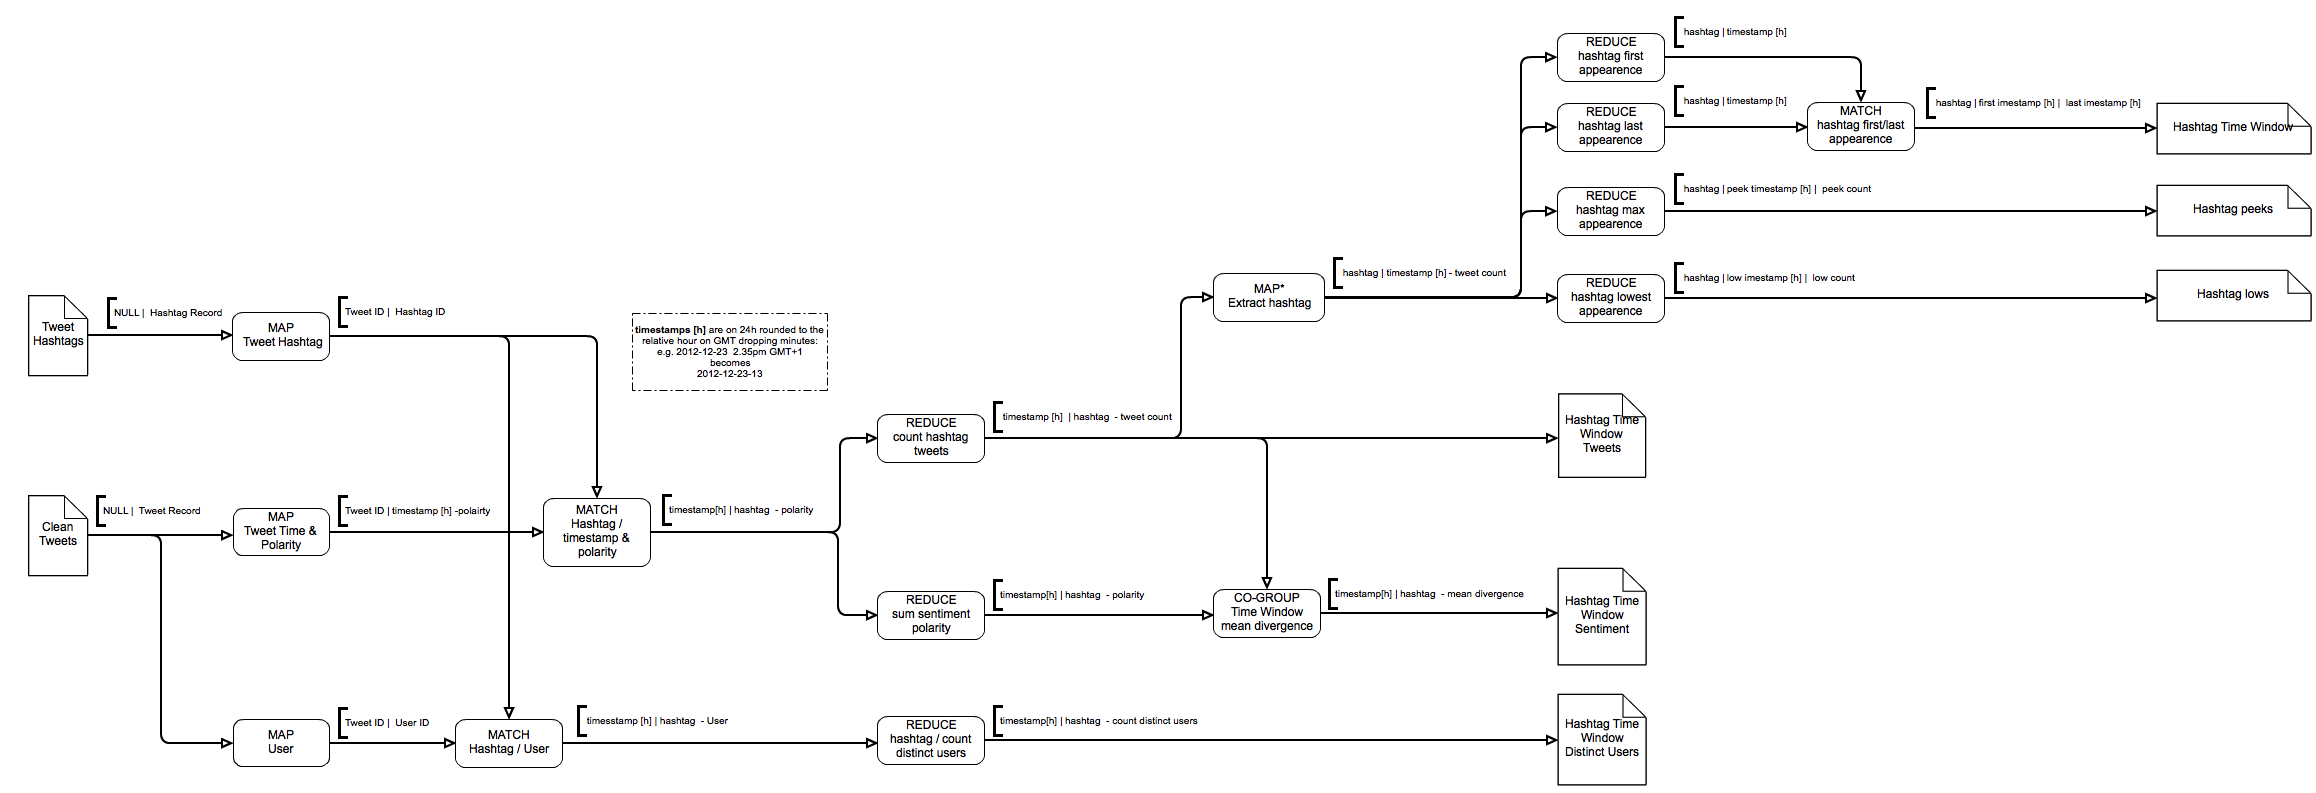
\includegraphics[width=\textwidth]{images/strato_pact_pt2.png} 
\caption{Compute statistics PACT}
\label{fig:statistics}
\end{figure*}

\section{Data}
\label{sec:data}

We downloaded 33 milion of English tweets from the tweet-stream using the streaming APIs\footnote{\url{https://dev.twitter.com/docs/streaming-apis}} on a period of approximately two weeks from December 18, 2012 to January 18, 2013~\footnote{We didn't downloaded any data durig the week between the 25-12-2012 and the 2-1-2013}. 
A summary of the main characteristic of the dataset is represented in table~\ref{tbl:dataset}.
The number of users is 16 milion, with an average of 2 tweets per user. 
The number of hashtags is one order of magnitude less than the number of tweets meaning that users often talk about same topics or do not mark their tweets with hashtags.
From this dataset we generated three datasets \textsc{100k-Tweets}, \textsc{1M-Tweets}, \textsc{10M-Tweets} with 100 thousands,1 million and 10 million tweets respectively, in order to test performance with various sizes of the dataset. 
We also downloaded a dictionary of 213 thousands English words to filter the meaningful tweets from those irrelevant or containing only symbols. 
To perform the sentiment analysis and (i.e., to assign a positive or negative polarity to the tweets) we used the SentiStrength library registering both positive and negative polarity carried in each tweet. 

\begin{table}[htb]
\centering 
\begin{tabular}{|l|r|}
\hline		
Period			& 2012-12-18/2013-01-18\\
\hline
Tweets			&	33774428\\
Users 			&	16099129\\
Hashtags 		&	1194691\\
Max tweets per user & 2380\\  
\hline
\end{tabular}
\caption{Characteristics of the dataset used in the experiments}
\label{tbl:dataset}
\end{table}


\section{Experimental evaluation}
\label{sec:results}
\begin{figure*}[!Ht]
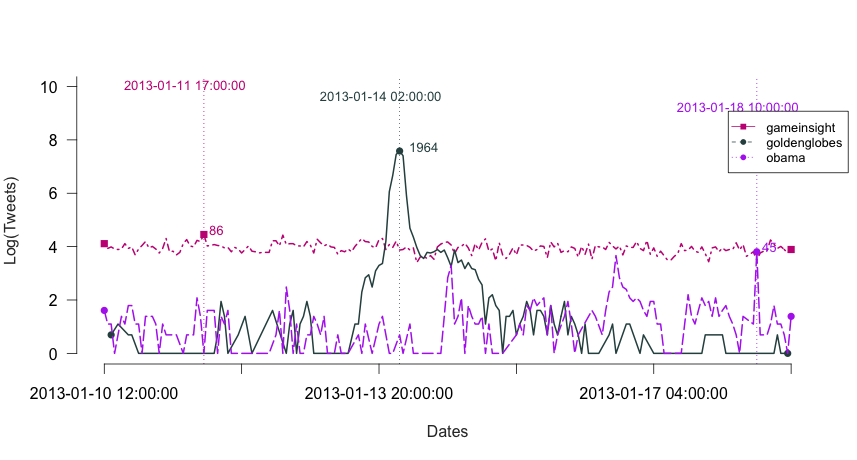
\includegraphics[width=0.9\textwidth]{images/3-plots.png} 
\caption{Popularity over time of three hashtags: gameinsight, goldenglobes and obama. Number of tweets have been normalized through the \emph{log} function}
\label{fig:trends}
\end{figure*}

\begin{figure}[!ht]
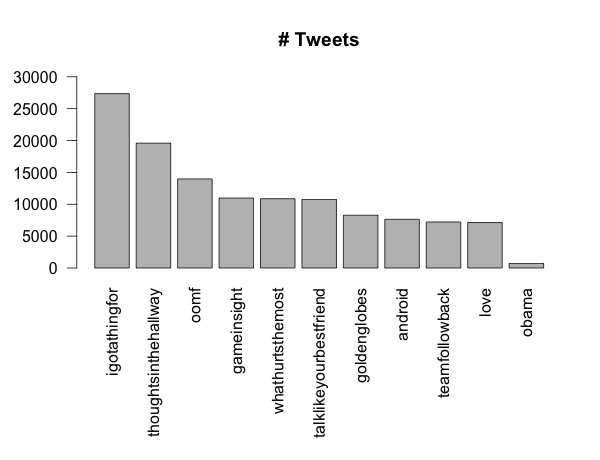
\includegraphics[width=0.45\textwidth]{images/hashtag-tweets-hist_20.png} 
\caption{Top10 hashtags for popularities within tweets, plus the hashtag for ``obama'' vs the number of tweets in which they appear}
\label{fig:tweets-hist}
\end{figure}

\begin{figure}[!ht]
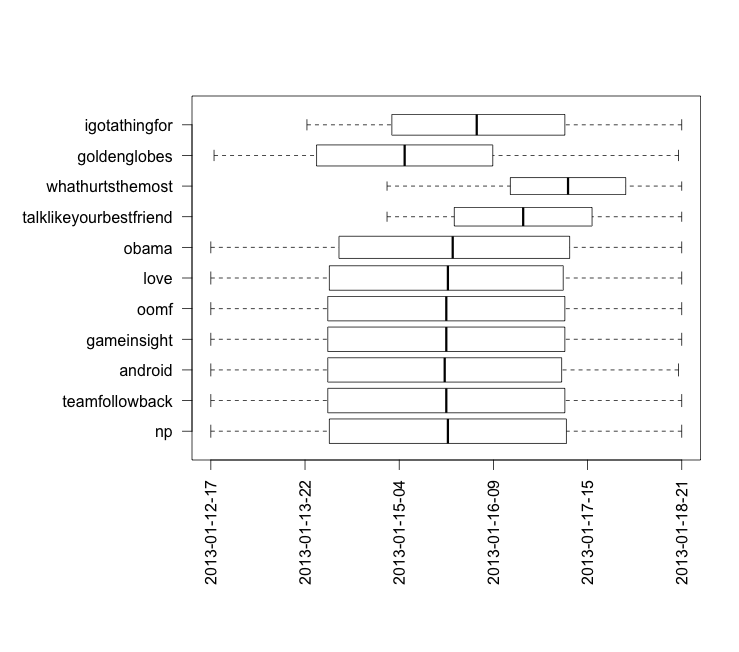
\includegraphics[width=0.45\textwidth]{images/hashtags-timewindow.png} 
\caption{Lifespan of the Top10 hashtags plus ``obama'' the thicker line delimits where the first and third quartile of tweets for that hashtag lies}
\label{fig:tweets-lifespan}
\end{figure}


We tested our solution with Stratosphere 0.2.1\footnote{\url{https://stratosphere.eu/downloads}} running on a GNU/Linux machine with 2Gb RAM DDR2, and a CPU AMD Athlon\texttrademark 64bit X2 Dual Core Processor 5000+.%\footnote{Linux 3.0.0-12-generic \#20-Ubuntu SMP x86\_64}. 
We used a version of Stratosphere which is not publicly available at the time of writing as still in beta-testing.
%Bugs present in the current implementation limited the degree of parallelism to 1.

All the experiments have been performed on samples of the original database, in order to show time and quality performance. 
We used Java JRE 1.6.0\_26 to program the PACT using the Stratosphere libraries and server, additionally we integrated the SentiStrength java library\footnote{\url{http://sentistrength.wlv.ac.uk}}. 
We performed preliminary experiments to set the english word threshold and we finally set it to $\sigma=0.1$, i.e., requiring at least 1 word out of ten being a valid English word.
%, in order not to prune too many tweets. 
Since we are matching with english words that are not stemmed a larger threshold would have pruned interesting tweets.  

\subsection{Time performance}
%Describe the time over the (number of threads [if we could]? size of the database)
In this section we briefly report and comment time performance registered in the various experiments.
We performed a total of 4 different experiments testing the flow on different dataset sizes. 
%, where the flow and so the statistics retrieved where always the same, but we changed the set of tweet over which we computed them.

%As said before we performed this experiment with a degree of parallelism se to 1.
%This means that Stratosphere had been instructed to compute each step sequentially without exploiting possible parallel computations.
In particular we run over the last 100 thousands, 1 million, 10 million and 20 million tweets, in reverse chronological order.
Time results are present in table~\ref{tbl:times}. 

As expected, we registered time performance rapidly increasing with respect to the number of tweets.
Although the dataset is big and the computed statistics are complex we measured a total time of at most 1 hour for 20 millions tweets in the worst case.

\begin{table}[htb]
\centering 
\begin{tabular}{|l|r|}
\hline		
Number of Tweets			& Time (secs)\\
\hline
$100$ thousands tweets		&	50\\
$1$ million tweets		& 183\\
$10$ million tweets 		& 1516\\
$20$ million tweets 		& 4006\\  
\hline
\end{tabular}
\caption{Time performances for the computation of the statistics with respect to the size of the dataset analyzed}
\label{tbl:times}
\end{table}


\begin{table}[htb]
\centering 
\begin{tabular}{|l|r|}
\hline		
Hashtag			& Number of Tweets\\
\hline
obama		&	1771\\
obamacare		& 173\\
nobama 		& 120\\
impeachobama 		& 73\\  
obama2012 		& 63\\  
\hline
\end{tabular}
\caption{Hashtags referring to ``Barack Obama'' and the number of tweets containing them}
\label{tbl:obama-tweets}
\end{table}

\subsection{Output charts}
% describe how we used the data and which parameters we extract. 
%As described previously, the scope of this work is building a flow that can cope with a large amount of tweets, and which can parse, clean and filter them.
%Moreover this flow is designed to compute and aggregate statistics for the hashtags present in the flow and can be extended  to many more analysis.
Starting from our initial assumption, i.e., hashtags  are indicators of events or discussion topics, we experimentally show how our PACT flow can find important patterns in our data.

\begin{figure*}[!Ht]
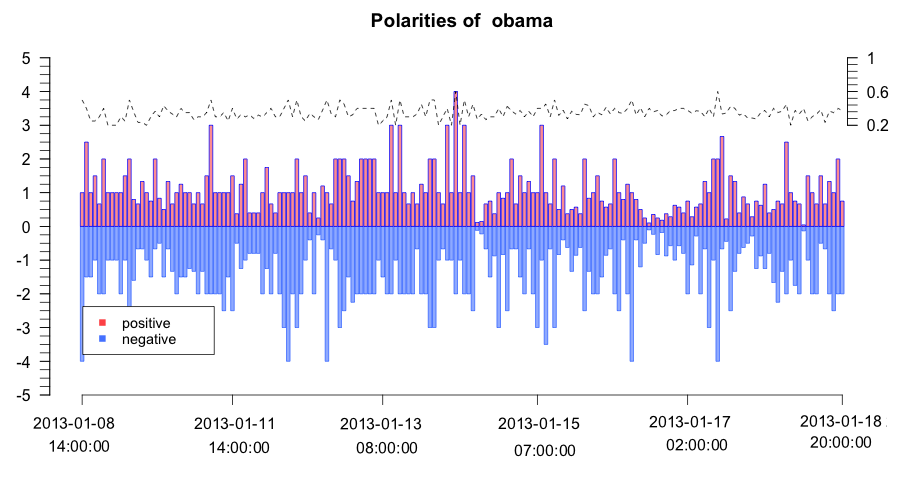
\includegraphics[width=0.9\textwidth]{images/obama-sentiment.png} 
\caption{Sentiment polarity expressed through tweets containing the hashtag ``obama''. The dashed line on the top, represent in each point in time the average emotional divergence.}
\label{fig:obama-sentiment}
\end{figure*}


In Figure~\ref{fig:tweets-hist} we show the Top10 hashtags for popularity, plus the hashtag for ``obama'' as a possibly interesting case  and we analyze their lifespan in Figure~\ref{fig:tweets-lifespan}.
Indeed, identifying that an hashtag has a limited lifespan within the flow of tweets may provide anecdotal evidence of an event happening in that  particular time window.
Looking instead to the hourly evolution of the popularity of each tweet we can identify interesting trends, points of peeks and lows.
In Figure~\ref{fig:trends} we can see how the popularity of some hashtags (expressed as hourly number of tweets), can have very different evolutions.
In that figure the hashtag ``gameinsight'' refers to the name of one developer and publisher of mobile games and social games, they and their followers use this hashtag when referring to some of these games.
We can see that during the time of the analysis the number of tweets mentioning this tag each our is pretty stable.
Instead, the other two hashtags have some highly unstable behavior.
The one referring to Barack Obama is not so much popular, even considering all the possible hashtags talking about president Obama, as we shown in Figure~\ref{tbl:obama-tweets}.
In contrast to the previous hashtag, the hourly number of tweets containing the tag ``obama'' is more unstable, and we can see that there are time windows where this number is actually zero.
Finally, in Figure~\ref{fig:trends} , we analyze also tweets regarding the ``goldenglobe'' hashtag, referring to the annual Golden Globe Awards, held in 2013 on the night of 13Th. of January.
The data-peak we can observe is an indicator of when the award night where held exhibiting a burst in the trend.
%, and we can easily see how before and after that peek was and returned to be pretty low.

Finally, another information to take into account, about the evolution of an event, is the polarity expressed in tweets about it.
In Figure \ref{fig:obama-sentiment} and ~\ref{fig:game-sentiment} we show average emotional polarities present in tweets in the hourly time-window.
These pictures demonstrates how while tweets containing the ``gameinsight'' keyword are more popular, tweets tagged with the hashtag ``obama'' have a more strong weight in terms of sentiment polarities.
These statistics combined with the evolution of popularity of hashtags are starting points for more complex models and analysis.
They can be used to actually identify which hashtags in which time windows are likely to be indicator of events happening.
Furthermore, approaches like the ones presented in \cite{Vlachos:2004:ISP:1007568.1007586} can be applied not only to identify burst in popularity or in sentiment polarities, but also to identify overlapping bursts, i.e. bursts in popularity for different hashtags in the same time window, so that we can actually detected which hashtags may refer to the same event.

In the end of our process we are able to aggregate, for the biggest dataset at our disposal, statistics for  more than 480 thousands hashtags, keeping tweets from more than 604 thousands users over 247 time windows.
These aggregated statistics can easily be used as grounds for more complex and structured reasoning, but they are already able to highlight popular hashtags.


\begin{figure*}[!Ht]
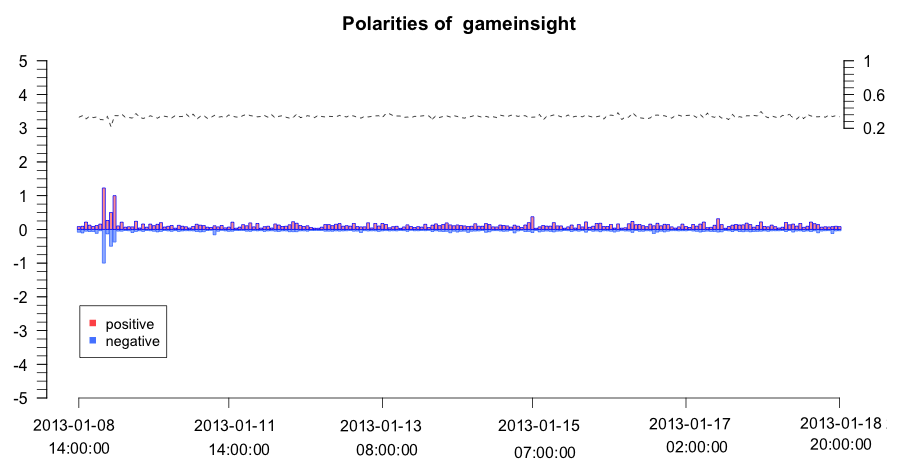
\includegraphics[width=0.9\textwidth]{images/game-sentiment.png} 
\caption{Sentiment polarity expressed through tweets containing the hashtag ``gameinsight''. The dashed line on the top, represent in each point in time the average emotional divergence.}
\label{fig:game-sentiment}
\end{figure*}






\section{Issues and conclusions}
\label{sec:issues}

\bibliographystyle{abbrv}
\bibliography{paperbib}  

\clearpage
\appendix
\section{PACT flow}

\vspace*{3cm}
\begin{figure}[h]
\centering
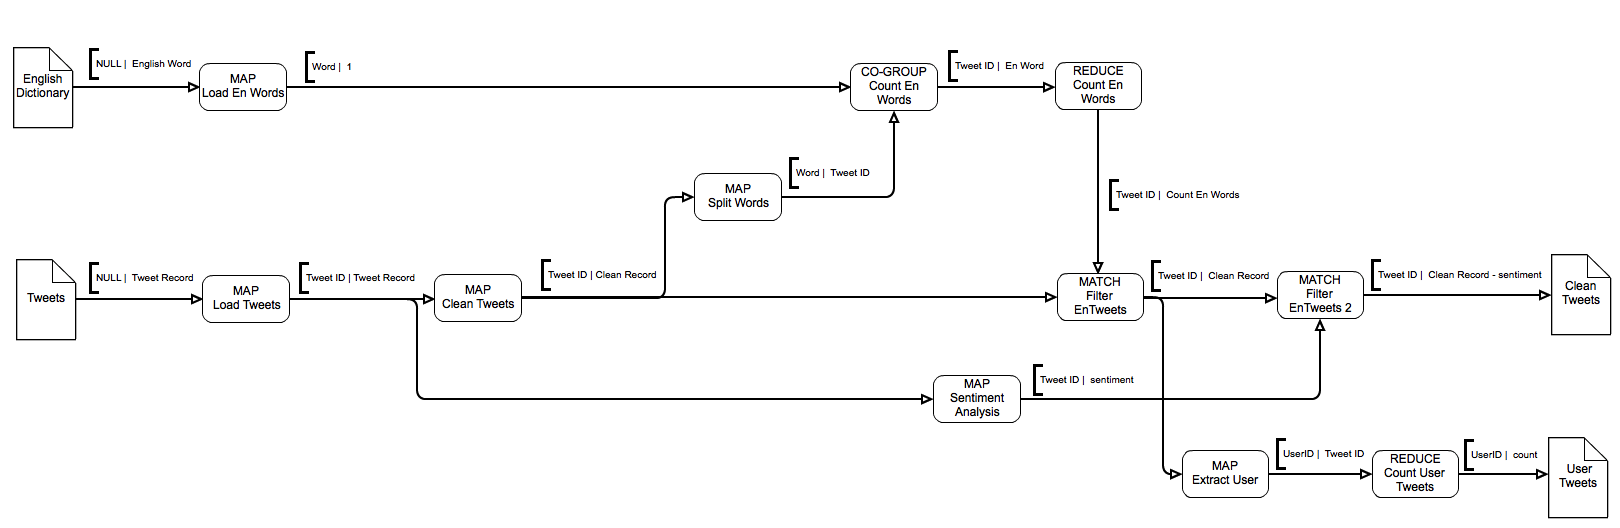
\includegraphics[angle=90,height=0.75\textheight]{images/strato_pact_pt1.png} 
\caption{Data cleaning PACT}
\label{fig:cleaning}
\end{figure}

\begin{figure}[h]
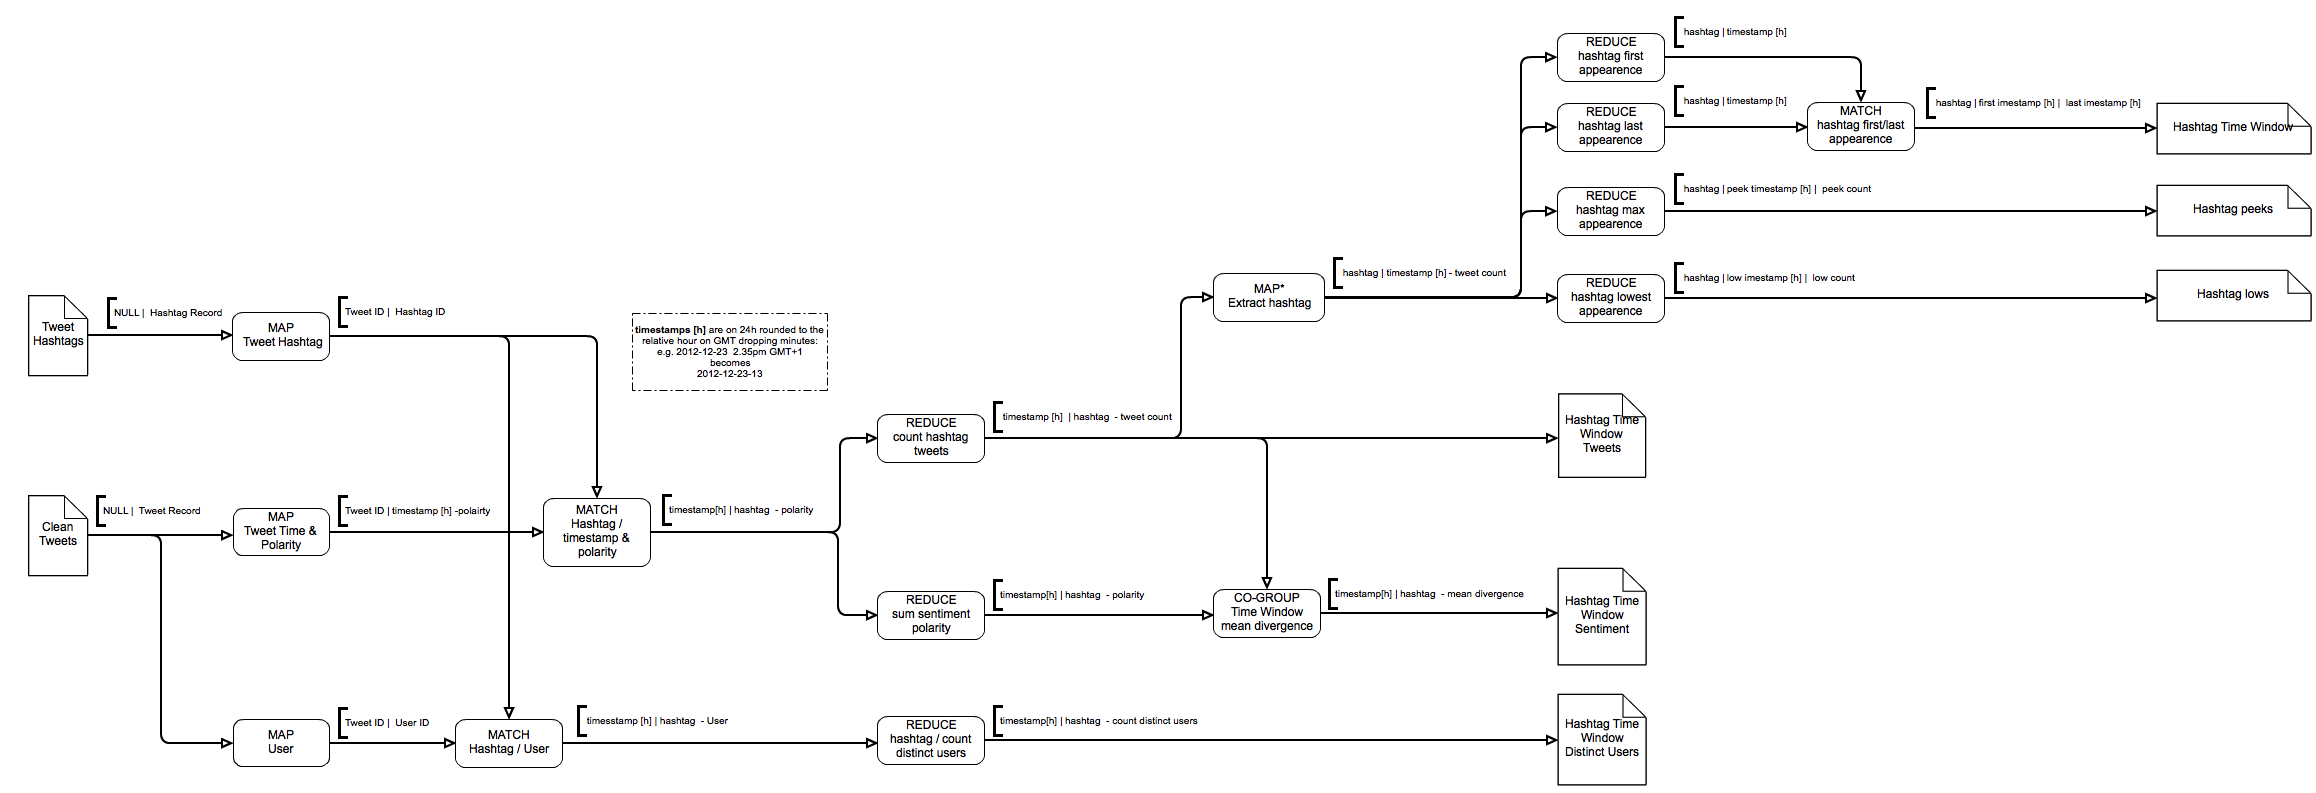
\includegraphics[angle=90,height=0.9\textheight]{images/strato_pact_pt2.png} 
\caption{Compute statistics PACT}
\label{fig:statistics}
\end{figure}

%\clearpage

%\def\thebibliography#1{
%  \section*{References}
% %\normalsize                  % smaller; put \normalsize after bib --dt
% %\small
% \scriptsize
%  \list
%    {[\arabic{enumi}]}
%    {\settowidth\labelwidth{[#1]}
%     \leftmargin\labelwidth
%     \parsep 1pt                % tighter --dt
%     \itemsep 0.6pt               % tighter --dt
%     \advance\leftmargin\labelsep
%     \usecounter{enumi}
%    }
%  \def\newblock{\hskip .11em plus .33em minus .07em}
%  \sloppy\clubpenalty10000\widowpenalty10000
%  \sfcode`\.=1000\relax
%}



\end{document}
